\begin{figure}[H]
     \centering
     \begin{subfigure}[b]{0.49\textwidth}
         \centering
         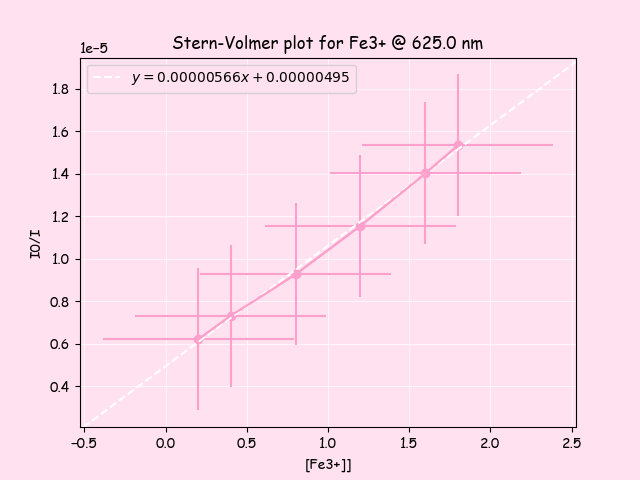
\includegraphics[width=\textwidth]{part1_q1_Fe.png}
         \caption{\ce{Fe^{3+}}}
         \label{fig:part1_q1_fe}
     \end{subfigure}
     \hfill
     \begin{subfigure}[b]{0.49\textwidth}
         \centering
         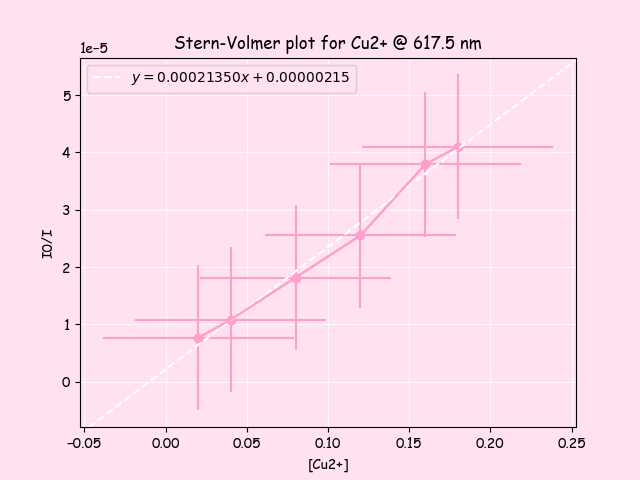
\includegraphics[width=\textwidth]{part1_q1_Cu.png}
         \caption{\ce{Cu^{2+}}}
         \label{fig:part1_q1_Cu}
     \end{subfigure}
     \caption{Stern-Volmer plots for luminescent quenching measurements}
     \label{fig:stern_volmers}
\end{figure}